\subsection{内存分配}

内存的分配方式涉及到内存释放,好的分配方式会使得内存使用的效率大大提高。
根据内存的大小来划分内存如何使用,预计使用32KB用于内存分配的管理空间,
则共有4000组左右的内存用于分配给各个程序使用,每个组4KB。

每一组内存经过初始化都拥有自己的数据结构,
即每一组空闲内存的地址和大小都被记录到空闲内存表free。

\begin{table}[!ht]
  \centering
  \begin{tabular}{|c|c|}
    \hline 组号 & 地址 \\
    \hline 2 & 0x00005000 \\ 
    \hline 1 & 0x00004000 \\
    \hline 0 & 0x00003000 \\
    \hline
  \end{tabular}
  \caption{空闲内存表free}
  \label{tab:free}
\end{table}

一旦系统接收到程序申请内存的请求(需求的内存大小),
就开始在内存中寻找足够大的内存完成这次申请,并返回可供使用的空闲内存的地址。
完成申请后系统需要重新整理空闲内存表free,将可用内存组数减一,
将返回给程序空闲空间大小根据程序需求进行调整,并对剩余的可用内存表进行按地址升序整理。

\begin{listing}[H]
  \inputminted[tabsize=2, firstline=68, lastline=78,
  linenos=true]{c}{../ZOS/src/kernel/memory.c}
  \caption{分配内存}
  \label{.lstc:alloc}
\end{listing}

% ----------------------------

\subsection{内存释放}

为保证磁盘空闲空间尽可能少的碎片化,内存释放首先考虑的是使待释放空间与附近空闲空间进行合并。

具体分为三种情况:

\begin{description}
\item[前端空闲:]释放内存的相连前端是空闲内存或释放内存相连两端都是空闲内存
\item[后端可用:]释放内存的相连后端是空闲空间
\item[前端后端均不可用:]在当前位置释放内存
\end{description}

已知:待释放的空间的地址和空间大小

根据空闲内存表free的编号从0到frees遍历查找地址大于待释放空间的空闲内存,
并根据得到的空闲内存编号i及大小size区分此时的待释放内存应当采取何种方式释放。
\begin{listing}[H]
  \inputminted[tabsize=2, firstline=91, lastline=95,
  linenos=true]{c}{../ZOS/src/kernel/memory.c}
  \caption{确定采取何种方式释放内存}
  \label{lst:rw}
\end{listing}

前端空闲:

当相连前端有可用内存时将可释放内存大小归入前端可用内存内,frees不变;

当相连后端也有可用内存时将后端内存大小归入前端可用内存内,frees减一。

\newpage
内存释放前后情况如图~\ref{fig:mem0}和图~\ref{fig:mem1}所示: 

\begin{figure}[h]
  \centering
  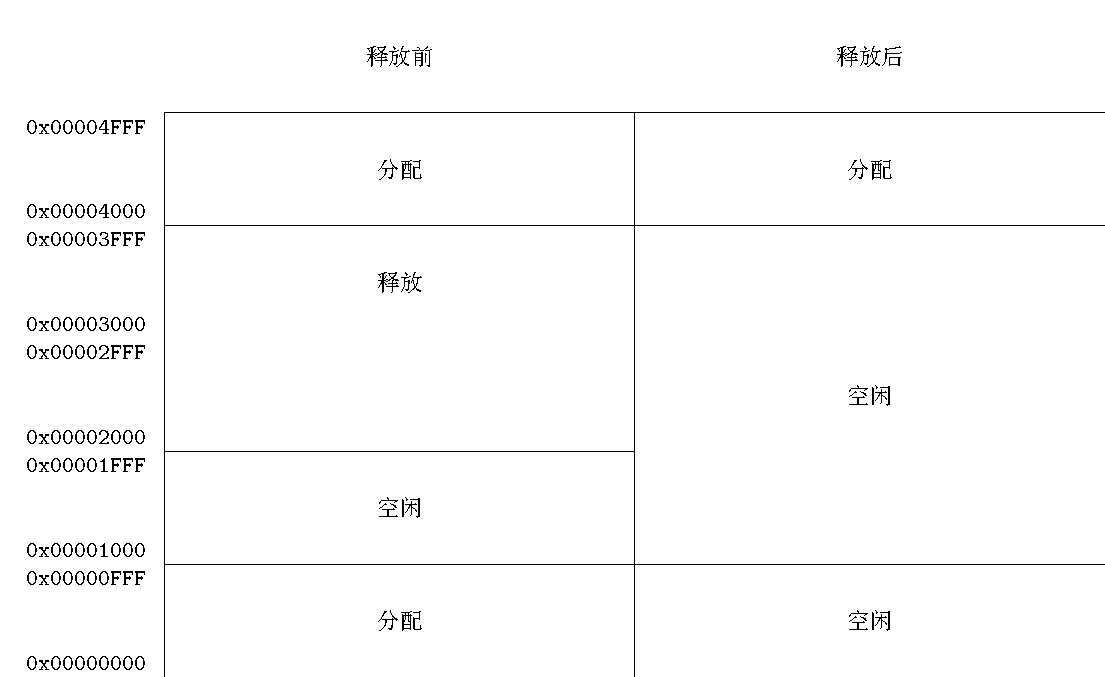
\includegraphics[width=.8\textwidth]{fig/mem0.pdf}
  \caption{前端空闲}
  \label{fig:mem0}
\end{figure}

\begin{figure}[h]
  \centering
  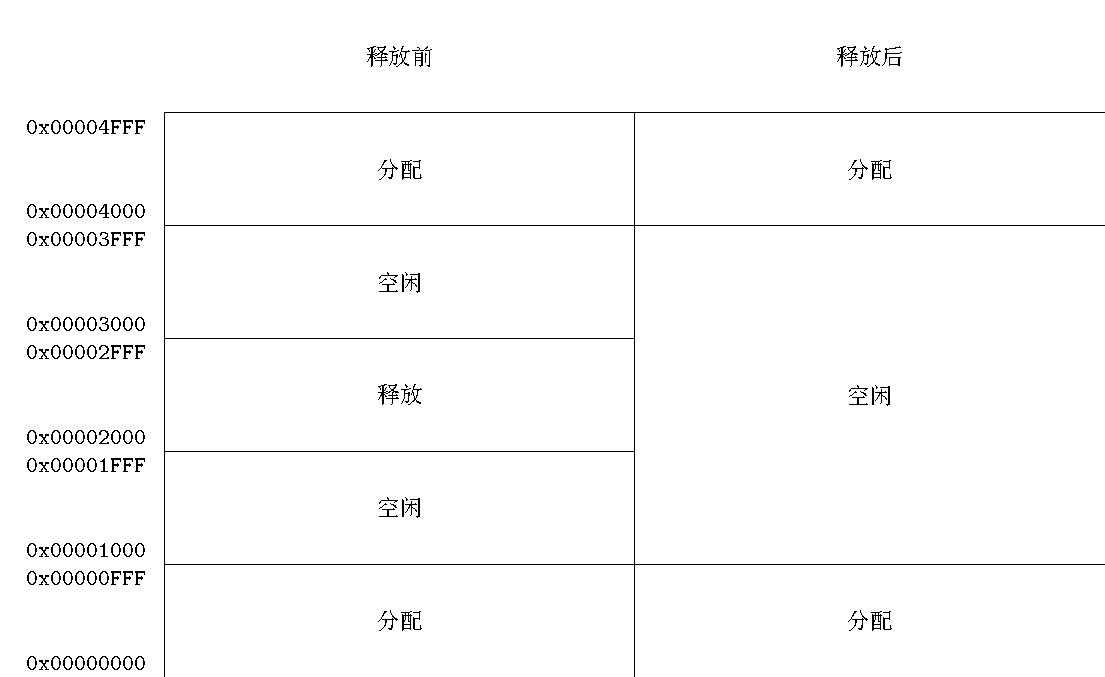
\includegraphics[width=.8\textwidth]{fig/mem1.pdf}
  \caption{前端可用,且后端空闲}
  \label{fig:mem1}
\end{figure}

\begin{listing}[H]
  \inputminted[tabsize=2, firstline=98, lastline=116,
  linenos=true]{c}{../ZOS/src/kernel/memory.c}
  \caption{前端可用}
  \label{lst:mem1}
\end{listing}

% ------------------------------

后端空闲:

内存释放前后情况如图~\ref{fig:mem2}所示:

当待释放的空间后方有空闲空间时,将free[i-1]的大小加上释放空间的大小
\begin{figure}[h]
  \centering
  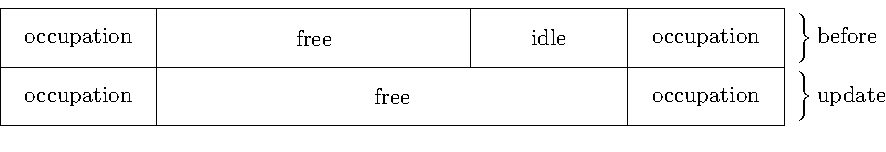
\includegraphics[width=.8\textwidth]{fig/mem2.pdf}
  \caption{后端空闲}
  \label{fig:mem2}
\end{figure}

当相连后端有可用内存的时候将free[i]的地址换为待释放内存的地址,相连后端内存大小归入待释放内存大小,frees不变。

\begin{listing}[H]
  \inputminted[tabsize=2, firstline=118, lastline=127,
  linenos=true]{c}{../ZOS/src/kernel/memory.c}
  \caption{后端空闲}
  \label{lst:mem2}
\end{listing}

% -----------------------------

前端后端均被占用:

由于被释放空间周围没有空闲内存,为保证free内各段内存仍然按照内存地址升序排列,
使空闲空间计数最大值加一,free[i]后续空闲内存序号加一,并将释放空间组号定为i。

\newpage
内存释放前后情况如图~\ref{fig:mem3}所示:
\begin{figure}[h]
  \centering
  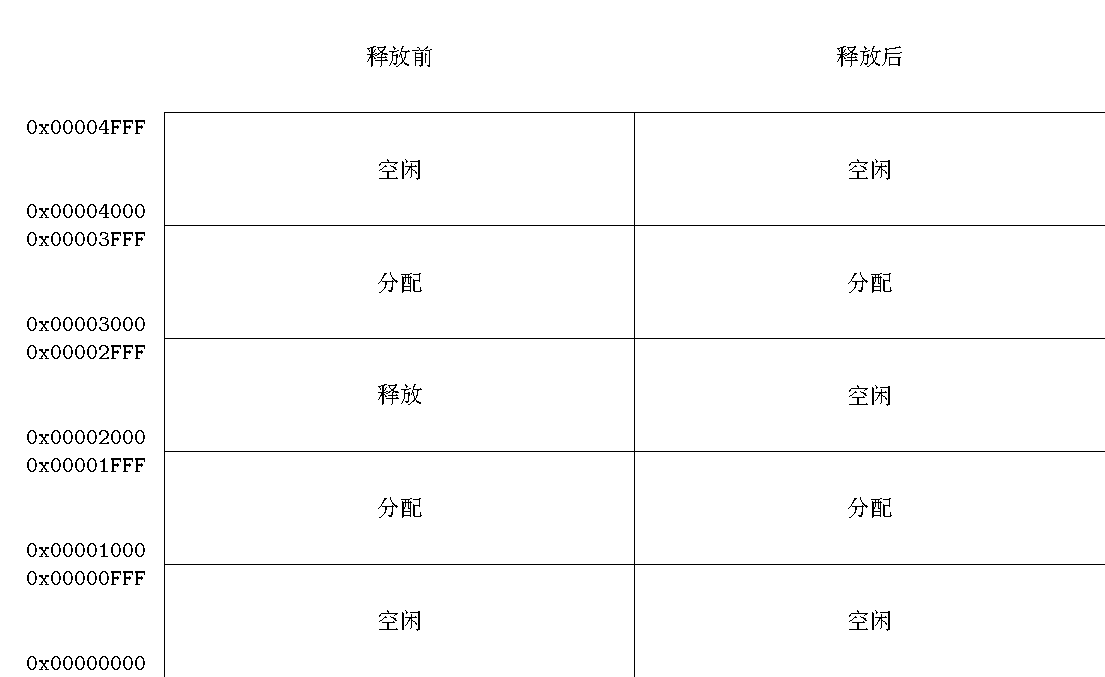
\includegraphics[width=.8\textwidth]{fig/mem3.pdf}
  \caption{前端后端均被占用}
  \label{fig:mem3}
\end{figure}

\begin{listing}[H]
  \inputminted[tabsize=2, firstline=128, lastline=141,
  linenos=true]{c}{../ZOS/src/kernel/memory.c}
  \caption{前端后端均被占用}
  \label{lst:mem3}
\end{listing}